\chapter{Consideraciones Especiales: Obst\'aculos y Soluciones} \label{chapter:consideraciones}

Durante el desarrollo del proyecto se presentaron algunos obst\'aculos que lograron ser resueltos. A continuación se describe la solución de algunos de esos obstáculos. 
\begin{itemize}
\item Errores de la tarjeta Arbotix para cargar programas:\\
	
	\textbf{Problema:} El IDE de Arduino 1.0.1 no funciona para quemar programar en la tarjeta Arbotix \\
  	\textbf{Soluci\'on:} Utilizar la versión 1.0.5 del IDE de Arduino  que compila los programas sin problema. \\
	

	 \textbf{Problema:} El gestor de arranque de la tarjeta Arbotix no estaba guardado.\\
	 \textbf{Soluci\'on:} Con el gestor de arranque de 'Sanguino' , se cargó a la Arbotix a través del    			    dispositivo programador para AVR llamado ' ISP programmer' que se muestra en la figura         \ref{fig:ISPprog}. 

	\begin{figure}[hbtp]
	\centering
	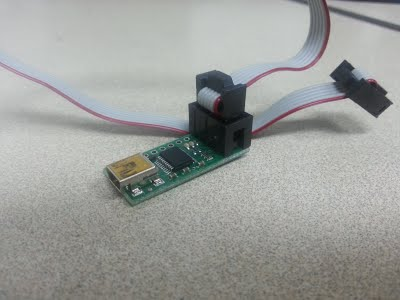
\includegraphics[scale=0.3]{imagenes/ISP.jpg}
	\caption{Programador para AVR.}
	\label{fig:ISPprog}
	\end{figure}
	
	

 \item Quema de Motores Dynamixel:\\

	\textbf{Problema:} Debido al uso prolongado pero necesario los motores Dynamixel AX-12 se dañaban, ya sea por motor DC o en chip interno.\\
	\textbf{Soluci\'on:} Fue controlar el torque y la temperatura máxima a la que pueden llegar los motores. En caso de llegar a estas cotas máximas los motores se apagan automáticamente. Las cotas máximas han sido de $30\deg$ centígrados para la temperatura y 800 kgf-cm para el torque. Para lograr esto se ha tenido que modificar la librería Ax12 agregando procedimientos que permitieran establecer la temperatura y el torque máximo.\\

En el archivo ax12.h se agregaron las siguientes definiciones de funciones:

\begin{lstlisting}

#define SetTemperature(id,temp) (ax12SetRegister(id,AX\_LIMIT\_TEMPERATURE, temp))
#define SetAlarm(id) (ax12SetRegister(id,AX\_ALARM\_SHUTDOWN, 0x04)) 
#define SetTorqueL(id, tor) (ax12SetRegister2(id,AX\_MAX\_TORQUE\_L, tor)) 
\end{lstlisting}
 

El archivo ax12.h viene con el paquete de la p\'agina oficial para el código de Arbotix. Como se indica en las instrucciones, este archivo se debe ubicar en la carpeta sketchbook de Arduino. Luego desde el IDE de Arduino llamamos a las funciones definidas con los valores deseados. De esta manera se ha solucionado el problema de la quema de motores.

\end{itemize}

\textbf{Recomendaciones}  

Para la instalación del sistema operativo Raspbian en la tarjeta Raspberry Pi se recomienda tener en cuenta que algunas tarjetas SD no funcionan adecuadamente. Si al prender la mini computadora solo se prende el led rojo, como ha ocurrido en este proyecto, se debe verificar que la tarjeta SD esta haciendo buen contacto con el puerto en que se conecta. Si se verifica esto último y aún asi no prende, es probable que se deba intentar con otra tarjeta SD. Al inicio de este proyecto se ha usado una tarjeta mini-SD de 32GB, como no ha funcionado se ha reemplazado con una tarjeta SD de 4GB. Esta última ha funcionado, sin embargo se ha quedado sin capacidad de almacenamiento al instalar OpenCV, por lo que se ha reemplazado nuevamente por una tarjeta SD de 16GB. Esta ha sido suficiente para instalar todo lo necesario con holgura.    

Como no se contaba con un monitor con entrada HDMI o VGA se debió buscar una solución alterna para observar la interfaz gráfica de Raspbian de la Raspberry Pi. Se utilizó el programa TightVNC para la visualización y control de la interfaz de Raspbian desde un computador remoto. Ha sido necesario poder observar lo que el robot percibe para llevar un control y una supervisión de su comportamiento. 

Por último, sería conveniente advertir que para la instalación de ROS en la Raspberry Pi, la versión que se debe obtener es la más reciente, de lo contrario podrían ocurrir problemas de sincronización en la comunicación de las tarjetas.   



